\documentclass{article}
\usepackage[utf8]{inputenc} 
\usepackage{Sweave}
\begin{document}
\Sconcordance{concordance:Example.tex:Example.Rnw:%
1 2 1 1 0 3 1 1 2 1 0 1 3 3 1 1 2 3 0 1 2 1 1 1 4 2 0 1 2 1 0 2 1 5 0 1 %
3 3 1}


O código abaixo serve para ler e formatar o CSV com os dados.
\begin{Schunk}
\begin{Sinput}
> setwd("~/Tese/Tese/Databases/CSV/Data")
> joaquim <- read.csv("Joaquim.csv")
> joaquim[is.na(joaquim)] <-0
> joaquim$Day <- weekdays(as.Date(joaquim$DateTime))
> joaquim$Period <- format(as.POSIXlt(joaquim$DateTime),"%H:%M:%S")
> joaquim$Period <- as.POSIXct(joaquim$Period, format="%H:%M")
\end{Sinput}
\end{Schunk}

O código abaixo serve para criar um gráfico de pontos .
\begin{Schunk}
\begin{Sinput}
> plot(joaquim$Period, joaquim$Value_Glucose, xaxt="n",
+      ylim=c(0,350), ylab="Valor de glicose", xlab="Hora")
> axis.POSIXct(1, joaquim$Period, seq(from=as.POSIXct("2016-02-13 0:00"), 
+      to=as.POSIXct("2017-02-20 23:00"), by="hour"), format="%H:%M")
> abline(h=70, col="red")
> abline(h=150, col="blue")
> 
\end{Sinput}
\end{Schunk}
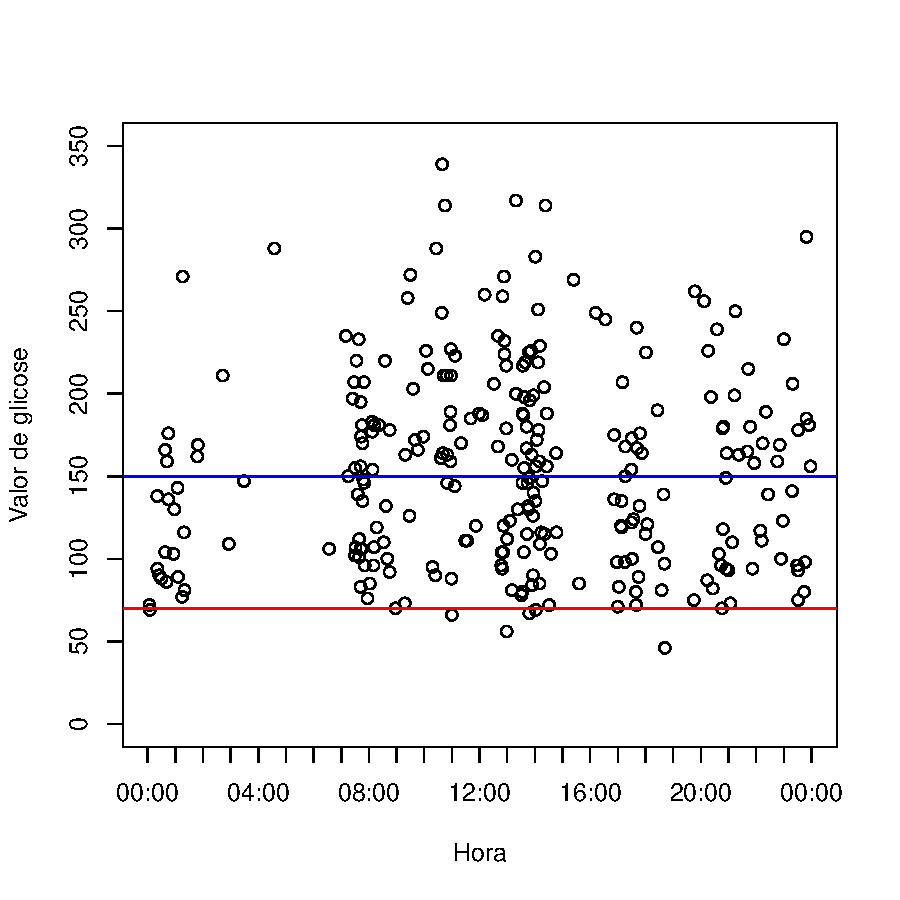
\includegraphics{Example-002}



\end{document}
